\documentclass[border=2mm]{standalone}
\usepackage{tikz}
\usetikzlibrary{calc}

\begin{document}
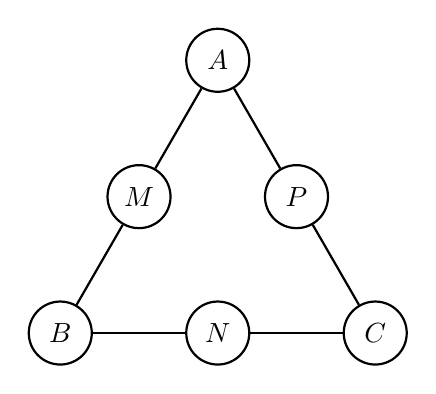
\begin{tikzpicture}[
    node/.style={circle, draw, minimum size=8mm, thick},
    edge/.style={draw, thick}]
    
% Kích thước tam giác
\def\side{4} % Độ dài cạnh
\def\height{3.464} % Chiều cao tam giác đều (sqrt(3)/2 * side)

% Định nghĩa 3 đỉnh
\coordinate (B) at (0,0);
\coordinate (C) at (\side,0);
\coordinate (A) at (\side/2,\height);

% Node tại các đỉnh
\node[node] (A-node) at (A) {$A$};
\node[node] (B-node) at (B) {$B$};
\node[node] (C-node) at (C) {$C$};

% Node tại trung điểm các cạnh
\node[node] (AB-mid) at ($(A)!0.5!(B)$) {$M$};
\node[node] (BC-mid) at ($(B)!0.5!(C)$) {$N$};
\node[node] (CA-mid) at ($(C)!0.5!(A)$) {$P$};

% Vẽ các cạnh tam giác
\draw[edge] (A-node) -- (AB-mid);
\draw[edge] (AB-mid) -- (B-node);
\draw[edge] (B-node) -- (BC-mid);
\draw[edge] (BC-mid) -- (C-node);
\draw[edge] (C-node) -- (CA-mid);
\draw[edge] (CA-mid) -- (A-node);

% \draw[edge] (A) -- (B);

\end{tikzpicture}
\end{document}